\documentclass[11pt,a4paper]{article}

\usepackage{amsmath}
\usepackage{amssymb}
\usepackage[english]{babel}
\usepackage[utf8]{inputenc}
\usepackage{multicol}
\usepackage[cm]{fullpage}
\usepackage{comment}
\usepackage[pdftex]{graphicx}
%\usepackage{GFS artemisia}
%\usepackage{verbatim}
\usepackage{tikz}
\usepackage{listings}
\usepackage{bm}
%\usepackage{sbbm}
\usepackage{float}
\usepackage{mathtools}
%\usepackage{subfigure}
\usepackage{fancyhdr}
\usepackage{simplewick}
\usepackage{slashed}
\usepackage{xfrac}
%\usepackage{tikz-feynman}

\usepackage[pass]{geometry}
%\usepackage{graphicx}
\usepackage{caption}
\usepackage{subcaption}

% % % Pagestyling
\pagestyle{fancy}
\fancyhf{}
\headsep = 25pt
% % %


% % % New commands
\newcommand{\HRule}{\rule{\linewidth}{0.5mm}}
\newcommand{\down}{\Big|\frac{1}{2}\:-\frac{1}{2}\Big\rangle}
\newcommand{\up}{\Big|\frac{1}{2}\:\:\:\:\frac{1}{2}\Big\rangle}
\renewcommand{\arraystretch}{1.5}
\newcommand{\bpm}{\begin{pmatrix}}
\newcommand{\epm}{\end{pmatrix}}

% % % Nice column vectors
\makeatletter
\newcommand{\Spvek}[2][r]{%
	\gdef\@VORNE{1}
	\left(\hskip-\arraycolsep%
	\begin{array}{#1}\vekSp@lten{#2}\end{array}%
	\hskip-\arraycolsep\right)}

\def\vekSp@lten#1{\xvekSp@lten#1;vekL@stLine;}
\def\vekL@stLine{vekL@stLine}
\def\xvekSp@lten#1;{\def\temp{#1}%
	\ifx\temp\vekL@stLine
	\else
	\ifnum\@VORNE=1\gdef\@VORNE{0}
	\else\@arraycr\fi%
	#1%
	\expandafter\xvekSp@lten
	\fi}
\makeatother
% % %

% % %

\renewcommand*\thesubfigure{\arabic{subfigure}}
\renewcommand{\labelenumii}{\theenumii}
\renewcommand{\theenumii}{\arabic{enumii}.}
\renewcommand{\labelenumiii}{\theenumiii}
\renewcommand{\theenumiii}{\arabic{enumiii}.}

% % % Enables Matlab-scipt import
\lstset{
        language=Matlab,                            
        numbers=left,                               
        numberstyle=\footnotesize,                  
        stepnumber=1,                               
        numbersep=5pt,                              
        showspaces=false,                           
        showstringspaces=false,                     
        showtabs=false,                             
        breaklines=true,                            
        breakatwhitespace=false,
        frame=single,
        commentstyle=\color{green},
        keywordstyle=\color{blue},
        escapeinside={\%*}{*)}  }
% % %

\begin{document}

% % % Titlepage start
\begin{titlepage}
\begin{center}
\medskip
\textsc{\LARGE FYS4560;}\\[0.3cm]
\textsc{\Large Elementary Particle Physics}\\[1.5cm]

\textsc{\Large Final Project}\\[0.5cm]

\HRule \\[1.0cm]
\textmd{ \huge Higher Dimensions; \\ \LARGE Theoretical and Experimental Aspects \\[0.4cm] }
\HRule \huge \\[1.5cm]

\begin{minipage}{0.4\textwidth}
\begin{center}
\large\textsc{Sean B.S. Miller}\\

\end{center}
\end{minipage}

\vfill

\begin{abstract}
	The Randall-Sundrum (RS) model of compacted dimensions will be studied, together with the postulate of the graviton particle. Quark-anti-quark production of the simplest possible massive graviton (1st order tower of Kaluza-Klein excitations) will be calculated.
\end{abstract}

\vfill

{\large \today}

\end{center}
\end{titlepage}
% % % Titlepage end

\newpage

\fancyhead[L]{\textsc{Final Project}}
\fancyhead[C]{\textsc{\today}}
\fancyhead[R]{\textsc{Sean B.S. Miller}}
\fancyfoot[C]{\thepage}

\section{Introduction}
Higher dimensions, also called extra dimensions, are physical models for the dimensionality of our universe, mostly suggested with the goal of explaining the hierarchy problem of the standard model. There are \emph{many} theories for higher dimensions. The most recognised are:
\begin{itemize}
	\item \emph{Large extra dimensions}: The often-heard theory that gravity acts through several dimensions, therefore becoming weaker. It originates from the ADD model as an attempt to solve the hierarchy problem\footnote{The "hierarchy problem" is the problem in explaining why gravity and the weak force are so weak compared to QED and QCD.}.
	\item \emph{Warped extra dimensions}: Describing our universe as a five-dimensional anti-de Sitter space, and claiming the SM particles are localized on a (3 + 1)-dimensional brane(s).
	\item \emph{Universal extra dimensions}: All particles move universally through the extra dimensions, unlike to two other models where only gravity propagates through them.
\end{itemize}

Obviously, a thorough description of any of these models is near impossible for such a small paper, let alone all the models together. Therefore, a brief outline of the theory behind the two currently most promising\footnote{"Promising" in the sense that they provide measurable outcomes, and fit very well with what we already know from the standard model. The problem is that so far they have predicted nothing. Finding a graviton would possibly confirm either theory.} models will be given.\\
The first is the large extra dimension model by Arkani-Hamed, Dimopoulos, and Dvali (ADD). Originally, it was proposed as a model to explain the hierarchy problem (why the weak force is $10^{32}$ times stronger than gravity, among other problems). The extra dimensions\footnote{Today, 6 dimensions is the most common expansion.} are then suggested as planes into which gravity, assumed just as strong as the other forces, spreads. Therefore gravity becomes "diluted", while the known SM particles stay in (1,3)-spacetime.\\
The second model is the warped extra dimension model by Randall and Sundrum (RS), made due to disliking the current universal extra dimensions models. They assumed that, rather than having universal extra dimensions in which all particles propagate,  there is a small extra dimension. This means they model our world as a 5-dimensional anti-de Sitter space\footnote{This will be explained later on.}. By small, it means the extra dimension has a large curvature, or is \emph{warped}. From general relativity, gravity and curvature are very much the same thing, and therefore the extra dimension, called the Planckbrane, can easily host gravitons.\\
A question that then springs to mind is why exactly gravitons and extra dimensions are connected (other than gravitons "carrying" gravity). If the standard model is expanded, but without inclusion of extra dimensions, to include a graviton field, then measuring it would be, at best, very optimistic\footnote{Refer to "Can Gravitons be Detected?" by Rothman and Boughn (https://arxiv.org/pdf/gr-qc/0601043v3.pdf) for an impression of the problem.}.
Should any extra dimensional model be true, it would certainly be desirable to prove it by measurement. Finding a particle with the properties of the graviton would mean that at least \emph{some} extra dimensions model is true.

\section{Kaluza-Klein theory}
The reason Kaluza-Klein theory is discussed is because one requires knowledge of the so-called "Kaluza-Klein towers"; massive excitations of an expansion model\footnote{This expansion depends on the model, and is where RS and ADD differ.} of the spacetime metric. While RS1 only considers a single extra dimension, ADD works for different numbers of dimensions. However, for the sake of simplicity, and comparison, only one extra dimension will be considered.\\
Before adding extra dimensions, the question of how get so-called "massive gravity"; a massive field carries the gravitational force. First, one starts with linearised gravity. Problems in general relativity can be approximated by perturbing Minkowski spacetime;

\begin{equation}
	g_{\mu\nu} = \eta_{\mu\nu} + h_{\mu\nu}
\end{equation}

where $g_{\mu\nu}$ is the approximated spacetime metric, $\eta_{\mu\nu}$ is the Minkowski metric, and $h_{\mu\nu}$ is the perturbation, and is what eventually was suggested to be gravitons. The Lagrangian density will then have a interactive term on the form $h_{\mu\nu}T^{\mu\nu}$, and a kinetic term for $h_ {\mu\nu}$. The field $h_{\mu\nu}$ can be given mass by saying the Lagrangian density also has a term $ah_{\mu\nu}h^{\mu\nu} + b(\eta_{\mu\nu}h^{\mu\nu})^2$. Markus Fierz and Wolfgang Pauli then, in 1939, wrote an article\footnote{Fierz, Markus; Pauli, Wolfgang (1939). "On relativistic wave equations for particles of arbitrary spin in an electromagnetic field". Proc. Roy. Soc. Lond. A173: 211–232.} in which they proved that $a=-b$ in order to avoid unphysical results. The result is the Fierz-Pauli Lagrangian for massive gravity\footnote{Note that this is \emph{not} the only way to get a massive gravity Lagrangian, and it has some problems as well. It serves well as an introductory example, however.} [SOURCE]:

\begin{equation}
	\frac{1}{\kappa^2}\sqrt{|g|}R = \frac{1}{4}\left( \partial^\mu h^{\nu\rho}\partial_\mu h_{\nu\rho} - \partial^\mu h^{\nu}_{\nu}\partial_\mu h^\rho_{\rho} - 2\partial^\nu h_{\nu\mu}\partial_\rho h^{\rho\mu} + 2\partial_\nu h^{\nu\mu}\partial_\mu h^{\rho}_{\rho} \right) + \mathcal{O}(\kappa)
	\label{eq:FierzPauli}
\end{equation}

Now, additional spatial dimensions may be added. These dimensions will not change the form of equation \ref{eq:FierzPauli}, so one can simply let indices change from greek to latin, i.e. $\mu\rightarrow a$, $\nu\rightarrow b$, etc..., where $a,b,\ldots \in \{4+d\}$. It is then assumed the perturbative field has a form

\begin{equation}
	\hat{h}_{ab} = 
	V_d^{-1/2}\begin{pmatrix}
	h_{\mu\nu} + \eta_{\mu\nu}\phi & A_{\mu i}\\
	A_{\nu j} & 2\phi_{ij}
	\end{pmatrix}
\end{equation}

where $V_d$ is the volume of the compactified space, $\eta_{\mu\nu}\phi$ is a Weyl rescaling and $A_{\mu i}$ is some tensor field. Since the fields are compact, one can claim periodicity of the field, such that a Fourier expansions is possible:

\begin{equation}
	h_{\mu\nu}(x,y) = \sum_{\substack{n=\{n_1,n_2,\ldots,n_5\}; \\ n_i\in\mathbb{Z}\:\forall\:i}} h_{n,\mu\nu}(x)Y_n(y)
\end{equation}

where $Y_n(y)$ are orthogonal, normalized eigenfuntions of the Laplace operator on the internal space\footnote{The extra dimension/space, denoted $K_d$.}:

\begin{equation}
\Delta_{K_d}Y_n(\theta) = \frac{\lambda_n}{R^2}Y_n(\theta)
\end{equation}

where $R$ is the "characteristic size" of the space $K_d$ (tied to the volume $V_d$). This series expansion is called the Kalulza-Klein (KK) tower of modes, and one value of $n$ is called mode $n$, and the corresponding term the $n$'th excitation. The field $h_{\mu\nu}(x,y)$ has to satisfy the d'Alembert equation, and in doing this one finds it necessary to redefine the fields $h_{\mu\nu}(x,y)$, $A_{\nu j}$, and $\phi_{ij}$, to $\tilde{h}_{n,\mu\nu}$, $\tilde{A}_{n,\mu i}$, and $\tilde{\phi}_{n,ij}$. The detailed steps are omitted, as they are many and non-intuitive. These new fields, when put into the Lagrangian, will give mass eigenstates. This redefinition of fields can be thought of as an analogue to the rotations from the CKM matrix in QCD theory (needed for mass eigenstates in the Lagrangian), but it is not the same (not a rotation). From the equation of motion one can go one to show that the masses are:

\begin{equation}
	m_n^2 = \frac{4\pi^2 n^2}{R^2}
\end{equation}

%%%
%\begin{equation}
%	\tilde{g}_{ab}(x,\theta) ) = 
%	\begin{pmatrix}
%		g_{\mu\nu}(x,\theta)-B_\mu(x,\theta) B_\nu(x,\theta) \Phi(x,\theta) & B_\mu(x,\theta)\Phi(x,\theta)\\
%		B_\nu(x,\theta)\Phi(x,\theta) & -\Phi(x,\theta)
%	\end{pmatrix}
%\end{equation}
%
%where
%\begin{itemize}
%	\item Latin indices represent all dimensions, greek indices represent 4-dimensional spacetime.
%	\item $g_{\mu\nu}$ is the 4-dimensional spacetime metric from before.
%	\item $B_\mu$ is a gauge field, defined by $B_\mu \equiv \frac{g_{\mu5}}{g_{55}}$
%	\item $\Phi$ is a scalar field, defined by $\Phi = g_{55}$.
%	\item $x$ are the normal spacetime coordinates, while $\theta$ is the extra coordinate. The notation is due to the extra dimension(s) often being "circular" (such as the $S^1$ space).
%\end{itemize}



%As can be seen, a complete description depends on $g_{\mu5}$ and $g_{55}$. However, this is precisely where the complication of extra dimensions arises. The metric depends on the space, and the shape of the space is what we do not know\footnote{This is why the field of extra dimensions can be so large and complex, as there are \emph{many} ways to guess at a shape of the new dimension(s), and each model gives a characteristic outcome which must fit experiments at, for example, the LHC.}. \\
%Firstly, consider a simple model with a massive scalar field $\hat{\phi}(x,\theta)$,
%
%\begin{equation}
%	S_5 = \int dx^4 d\theta \sqrt{-\tilde{G}}\left(-\frac{1}{2}(\partial_ a\hat{\phi})(\partial^a\hat{\phi})^\dagger - \frac{m^2}{2}\hat{\phi}^2 - \frac{c_5}{4!}\hat{\phi}^4\right)
%	\label{eq:KKaction}
%\end{equation}
%
%where $\tilde{G} \equiv \det(\tilde{g}_{ab})$ and $c_5$ is some coupling constant we do not yet know. The scalar field can be Fourier expanded as
%
%\begin{equation}
%	\hat{\phi}(x,\theta) = \sum_{\substack{n=\{n_1,n_2,\ldots,n_5\}; \\ n_i\in\mathbb{Z}\:\forall\:i}} \phi{(n)}(x)Y_n(\theta)
%\end{equation}
%
%where $Y_n(\theta)$ are orthogonal, normalized eigenfuntions of the Laplace operator on the internal space\footnote{The extra dimension/space, denoted $K_d$.}:
%
%\begin{equation}
%	\Delta_{K_d}Y_n(\theta) = \frac{\lambda_n}{R^2}Y_n(\theta)
%\end{equation}
%
%where $R$ is the "characteristic size" of the space $K_d$ (obviously a radius in the case of circular objects).
%%%

%Inserting this into equation  and performing the integral over $K_d$ gives
%
%\begin{align}
%	\begin{split}
%	S_5 = \int dx^4 \sqrt{-\tilde{G}}\bigg(&-\frac{1}{2}(\partial_ \mu\phi^{(0)})(\partial^\mu\phi^{(0)})^\dagger - \frac{m^2}{2}\left(\phi^{(0)}\right)^2\\
%	& - \sum_{n\neq0} \left[(\partial_ \mu\phi^{(n)})(\partial^\mu\phi^{(n)})^\dagger + m_n^2\phi^{(n)}\phi^{(n)\dagger}\right]\\
%	& - \frac{c_5}{4!}\left(\phi^{(0)}\right)^4 - \frac{c_5}{4}\left(\phi^{(0)}\right)^2\sum_{n\neq0} \phi^{(n)}\phi^{(n)\dagger} - \ldots\bigg),
%	\end{split}
%\end{align}
%
%and by comparison one sees $m_n^2 = m^2 + \frac{\lambda_n}{R^2}$. The dots represent all terms without any $\phi^{(0)}$-coefficients. As one sees, there is an infinite number of masses, since there is an infinite number of eigenvalues; a mathematical problem without any current answer. The hope is that these modes\footnote{The infinite set of which is called the Kaluza-Klein tower of modes. (Often one hears of KK towers.)} can be tied to the graviton, and will be explained better in the following sections.\\
%%%


A relation that will be of importance later is the reduction formula:

\begin{equation}
	M_{Pl}^2 = V_dM^{d+2}
\end{equation}

where $M_{Pl} = G_{N(4)}^{-1/2}$ is the 4-dimensional Planck mass and $M^{d+2} = G_{N(4+d)}^{-1/(4+d)}$ is the fundamental mass scale in the new model. The relation is derived by demanding the Einstein-Hilbert action to be the same with and without the new dimension(s)\footnote{This is because the new dimension(s) must reproduce what we observe, and 4D spacetime fits very well with observations.}, and performing the integrals by using KK mode expansion on the integrand. I.e one demands:

\begin{equation}
	S_{E(4)} = S_{E(d+4)}
\end{equation}

where

\begin{equation}
	S_{E(D)} = \int d^D x\sqrt{-G_D} \frac{1}{16\pi G_{N(D)}}\mathcal{R}^{D}(G_{ab})
\end{equation}

With the principles of the KK tower and massive gravity, one can start to consider theories that are based on extra dimensions.\\
As is the point with Feynman diagrams, Feynman rules for the graviton would help do calculations. The propagator of massive, spin-2 KK excitations are given by the Fierz-Pauli equation of motion (see reference BLADIBLA), and is

\begin{equation}
	G_n^{\mu\nu\rho\sigma} = i\frac{\eta^{\mu\rho}\eta^{\nu\sigma} + \eta^{\mu\sigma}\eta^{\nu\rho} - \frac{2}{3}\eta^{\mu\nu}\eta^{\rho\sigma}}{k_G^2 - m_n^2 + i\epsilon}
	\label{eq:Gprop}
\end{equation}

The vertex factors with different fields (scalar, spinor, vector-boson) are found by inserting the conserved energy-momentum tensor, for said field, into the Lagrangian, except for the spinor-field. Spinor-graviton couplings, which will be of interest later on, must be found by using the vierbein formalism\footnote{A way with which to rewrite the spacetime metric. The details of this are many and unnecessary for purpose of this paper.}. The massive spinor-graviton spin-2 coupling is

\begin{equation}
	-\frac{i\kappa}{8}\left[\gamma_\mu(k_1 + k_2)_ \nu + \gamma_\nu(k_1+k_2)_\mu - 2\eta_{\mu\nu}(\slashed k_1 + \slashed k_2 - 2m_f)\right]
	\label{eq:Gcoupling}
\end{equation}

\section{The Arkani-Hamed-Dimopoulos-Dvali model}
The ADD model is mainly based on 3 features:

\begin{itemize}
	\item There exists $d$ new spatial compact dimensions, with compactification volume $V_d$.
	\item The Planck scale is very low, at the order of one TeV,
	\item The SM degrees of freedom are localized on a 3D-brane, stretching along 3 non-compact spatial dimensions (i.e. the SM particles move in normal spacetime, not in the new dimension(s)).
\end{itemize}

The idea is that the electroweak scale is the only fundamental scale in the universe, and that the true Planck scale is actually of the same order. from the reduction formula, one could introduce $d$ new spatial dimensions and find their size, i.e.

\begin{equation}
	\frac{M_{Pl}^2}{M^{d+2}} = V_d \sim R^d	\quad,\quad \mathcal{O}(M^{d+2}) = \mathcal{O}(m_{EW})
\end{equation}

where $R$ is the compactification radius as before. With new dimensions, Newton's law for gravitational force would instead be proportional to $r^{-(d+2)}$, which is of course not true. However, since the extra dimensions are compact, only objects with distances less $r<<R$ feel this new force, while it still goes as $r^{-2}$ for $r>>R$. Therefore, for $d=1$, the radius is of the same order as the earth-moon distance, and therefore $d$ can't be equal one. $d=2$ is not possible either. For $d>2$, the radius is so small that van der Waal forces prevent us from conducting "table-top" experiments, and is where particle physics experiments at CERN become relevant. If ADD is true, then it should be possible to determine the radius by measuring the graviton, which is a direct consequence of extra dimensions. Since the mass $m_n$ is inversely proportional to the size, it would be possible to determine the new Planck scale.

%In the ADD model, the standard metric is expanded upon by introducing a field $\hat{h}_{ab}(x,\theta)$ such that:
%
%\begin{equation}
%	\tilde{g}_{ab}(x,\theta) = \eta_{ab} + \frac{2}{M^{1+d/2}}\hat{h}_{ab}(x,\theta)
%\end{equation}

A problem with the massive KK spin-2 propagator is that there are infinitely many KK excitations, each with its own mass. When calculating a Feynman diagram, one has to, in principle, perform a sum over all modes, as one can't know which mode will appear.\\
In the ADD model, the masses are \emph{very} small, due to the size of $R$ by the reduction formula and the size of $M^{2+d}$, and evenly spaced. This means one can approximate the sum by an integral over the modes ($n$).

\section{The Randall-Sundrum model}
\subsection{The hierarchy problem in RS1}
The RS model assumes that there are two points on the $S^1/\mathbb{Z}^2$ ordibfold in which 3-branes are compactified. What this means is that there are two 3-dimensional, non-compact branes that are connected at every point by a "circle", see figure SOME FIG.\\



The two branes, 1 and 2, are located on points $\theta = 0$ and $\theta = \pi$, which means the branes are seperated by a distance $2L = 2R$, where $R$ is the circle radius.\\
As mentioned, the model set out to explain the hierarchy problem, and will be briefly explained how below. Firstly, the action of the model is given by the sum of the Hilbert-Einstein action and the "matter part":

\begin{equation}
	S_5 = S_E + S_M = \int d^4x \int_{-L}^{L} dy \sqrt{-\tilde{G}}(M^3\mathcal{R}_5 - \Lambda_5)
\end{equation}

where $\Lambda_5$ is the five dimensional cosmological constant. In order to match real world observations, the new metric must uphold Poinecaré invariance, which can be shown to lead to:

\begin{equation}
	ds^2 = e^{-2A(y)}\eta_{\mu\nu}dx^\mu dx^\nu + dy^2
	\label{eq:RS_lineelement}
\end{equation}

where $A(y)$ is called the \emph{warp factor}. Solving the Einstein equations lets one find that $A(y) = \pm ky$, where $k \equiv \sqrt{\frac{-\Lambda}{12M^3}}$ is a constant. Since the orbifold abides $\mathbb{Z}^2$ symmetry, $A(y) = A(-y) \:\rightarrow\: A(y) = k|y|$.\\
There is a problem with action above, which is that it does not include the energy densities of the two branes, that are:

\begin{align}
	S_1 &= \int_{B_1}\int_{S^1/\mathbb{Z}^2}d^4xdy \sqrt{-\tilde{G}(x,y)}\lambda_1\delta(y)\\
	S_2 &= \int_{B_2}\int_{S^1/\mathbb{Z}^2}d^4xdy \sqrt{-\tilde{G}(x,y)}\lambda_2\delta(y-L)
\end{align}

where $\tilde{G}(x,0) = G_1$ and $\tilde{G}(x,L) = G_2$ have been used. So, the total action for the space is $S = S_E+S_M+S_1+S_2$. To fulfil the Einstein equations, one needs to impose $\lambda_1 = -\lambda_2 = 12kM^3$. THINK ON THIS

\subsection{KK mode expansion/Finding gravitons}
Much in the same manner as for QED and other gauge theories, one can create gravitational bosons. This means doing a metric transform, given by:

\begin{equation}
	ds^2 = e^{-2k|y|}(\eta_{\mu\nu} + \tilde{h}_{\mu\nu}(x,y))dx^\mu dx^\nu + (1+\phi(x))dy^2
\end{equation}

However, this means there will be cross-terms ($\phi \tilde{h}_{\mu\nu}$-terms) in the Lagrangian that prevent mass eigenstates. It can be shown\footnote{See \text{http://arxiv.org/abs/hep-th/0105304v3}, section 2, for a rigorous derivation.} that it can be diagonalized. One will end up with two fields, $h_{\mu\nu}$ and $\varphi$, which will be used hereafter.\\
Then, a KK mode expansion is done on $h_{\mu\nu}(x,y)$, giving

\begin{equation}
	h_{\mu\nu}(x,y) = \sum_{n=0}^{\infty} h_{\mu\nu}^{(n)}(x)\frac{\chi_n(y)}{R},
\end{equation}

where $\chi_0(y) = 2\sqrt{kR}e^{-2k|y|}$ and

\begin{equation}
	\chi_n(y) = N_n\left[ C_1Y_2\left(\frac{m_n}{k}e^{k|y|}\right) +   C_2J_2\left(\frac{m_n}{k}e^{k|y|}\right)\right] \quad,\quad n\neq 0
\end{equation}

While this seems out of the blue, this is the result of diagonalizing the Lagrangian, which is a rather intricate procedure. The functions $\chi_n$ are eigenfunction of an equation met during the diagonalising of the Lagrangian. $J_2$ and $Y_2$ are the Bessel functions of the first and second kind, respectively. The constants $C_1$ and $C_2$ can be determined by the boundary conditions on the vacuum energy terms of the energy-momentum tensor (the delta functions),

\begin{equation}
	T_{ab} = \lambda_1\sqrt{G_1}g_{\mu\nu}^{(1)}\delta_a^\mu\delta_b^\nu\delta(y) + \lambda_2\sqrt{G_2}g_{\mu\nu}^{(2)}\delta_a^\mu\delta_b^\nu\delta(y-\pi R),
\end{equation}

which give $C_1 = Y_1\left(\frac{m_n}{k}\right)$ and $C_2 = -J_1\left(\frac{m_n}{k}\right)$ SOMETHING MORE HERE\\

The $h_{\mu\nu}^{(0)}(x)$ field describes the massless graviton, while the $n\geq 1$ states are the massive KK modes, and finally $\varphi$ describes the massless \emph{radion}.


\begin{figure}[H]
	\centering
	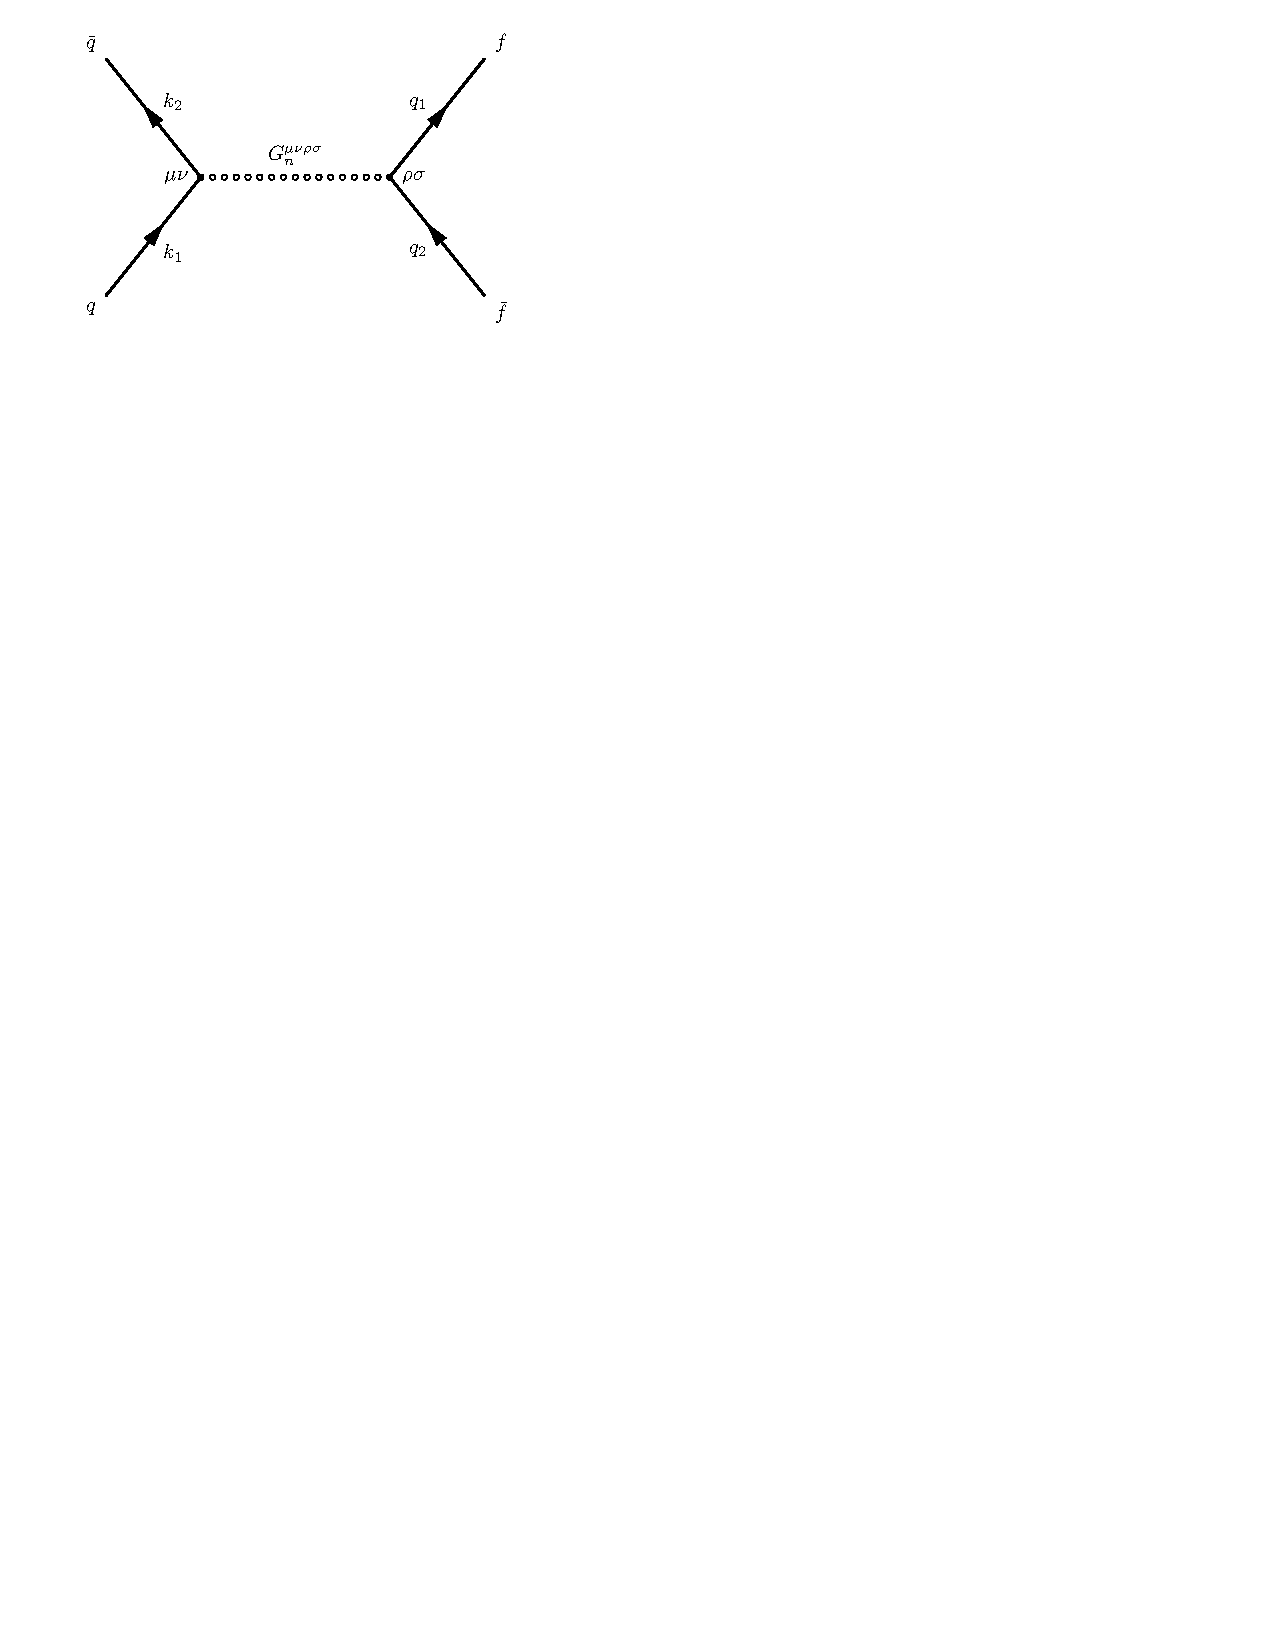
\includegraphics[trim={0.5cm 22cm 11.5cm 0cm},scale=1]{feynGraphs/qqbar_G_ffbar}
	\caption{$q\bar{q}\:\rightarrow\:f\bar{f}$}
	\label{fig:gravitonChannel}
\end{figure}

\section{Graviton production at the LHC}



\section{Conclusions}

\appendix
\section{Calculations}
A detailed calculation for the channel $q\bar{q}\:\rightarrow\:l^+l^-$ is as follows.\\
The $n$'th resonance spin-2 KK graviton propagator is given equation \ref{eq:Gprop}. The $G\bar{\psi}\psi$-coupling is given in equation \ref{eq:Gcoupling}.\\
The diagram shown in figure \ref{fig:gravitonChannel} therefore has effective amplitudes:

\begin{align}
	\begin{split}
	i\mathcal{M}(q\bar{q}\:\rightarrow\:f\bar{f}) = -\sum_{n}\frac{i\kappa^2}{64}\bar{u}_q&\left[\gamma_\rho(q_1 + q_2)_\sigma + \gamma_\sigma(q_1+q_2)_\rho - 2\eta_{\rho\sigma}(\slashed q_1 + \slashed q_2 - 2m_f)\right]v_q\\
	\times&\left[\frac{\eta^{\mu\rho}\eta^{\nu\sigma} + \eta^{\mu\sigma}\eta^{\nu\rho} - \frac{2}{3}\eta^{\mu\nu}\eta^{\rho\sigma}}{k_G^2 - m_n^2 + i\epsilon}\right]\\
	\times\bar{v}_k&\left[\gamma_\mu(k_1 + k_2)_\nu + \gamma_\nu(k_1+k_2)_\mu - 2\eta_{\mu\nu}(\slashed k_1 + \slashed k_2 - 2m_f)\right]u_k\\
	= -i\frac{\pi C_4}{4}\bar{u}_q&\left[\gamma_\rho(q_1 + q_2)_ \sigma + \gamma_\sigma(q_1+q_2)_\rho - 2\eta_{\rho\sigma}(\slashed q_1 + \slashed q_2 - 2m_f)\right]v_q\\
	\times\bar{v}_k&\left[\gamma^\rho(k_1 + k_2)^\sigma + \gamma^\sigma(k_1+k_2)^\rho + \frac{4}{3}\eta^{\sigma\rho}\right]u_k\\
	= -i\frac{\pi C_4}{2}\bar{u}_q&\Big[(q_1 + q_2)_ \mu(k_1+k_2)^\mu \gamma_\nu v_q\bar{v}_k\gamma^\nu + (\slashed k_1 + \slashed k_2)v_q\bar{v}_k(\slashed q_1 + \slashed q_2)\\
	&- 2(\slashed q_1 + \slashed q_2)v_q\bar{v}_k(\slashed k_1 + \slashed k_2) + 4\left(m_q(\slashed q_1 + \slashed q_2)v_q\bar{v}_k + m_fv_q\bar{v}_k(\slashed k_1 + \slashed k_2)\right)\\
	&- \frac{32}{3}m_fm_qv_q\bar{v}_k\Big]u_k
	\end{split}
\end{align}

 where $C_4 \equiv \frac{\kappa^2}{8\pi} D(s)$, $D(s) \equiv \sum_{n} \frac{1}{k_G^2 - m_n^2 + i\epsilon}$. The above expression can be rewritten as

\begin{align}
	\begin{split}
	i\mathcal{M}(q\bar{q}\:\rightarrow\:f\bar{f}) = -i\frac{\pi C_4}{2}\bar{u}_q\Big[&(q_1 + q_2)_ \mu(k_1+k_2)^\mu \gamma_\nu v_q\bar{v}_k\gamma^\nu + (\slashed k_1 + \slashed k_2)v_q\bar{v}_k(\slashed q_1 + \slashed q_2) - \frac{8}{3}m_fm_qv_q\bar{v}_k\\
	&-2(\slashed q_1 + \slashed q_2 - 2m_f)v_q\bar{v}_k(\slashed k_1 + \slashed k_2 - 2m_q)\Big]u_k
	\end{split}
\end{align}

The last term in the above equation is actually just the Dirac equation in momentum space,

\begin{equation}
	(\slashed k - m_f)u_f(k) = 0,
\end{equation}

and therefore equals zero. The amplitude is then

\begin{equation}
	i\mathcal{M}(q\bar{q}\:\rightarrow\:f\bar{f}) = -i\frac{\pi C_4}{2}\bar{u}_q\left[(q_1 + q_2)_ \mu(k_1+k_2)^\mu \gamma_\nu v_q\bar{v}_k\gamma^\nu + (\slashed k_1 + \slashed k_2)v_q\bar{v}_k(\slashed q_1 + \slashed q_2) - \frac{8}{3}m_fm_qv_q\bar{v}_k\right]u_k
\end{equation}

for the spin-2 massive KK graviton propagators.



\end{document}